\documentclass[journal]{new-aiaa}
\usepackage[utf8]{inputenc}

\usepackage{graphicx}
\usepackage{subcaption}
\usepackage{amsmath}
\usepackage[version=4]{mhchem}
\usepackage{siunitx}
\usepackage{float}
\usepackage{array}
\usepackage[export]{adjustbox}
\usepackage{longtable, tabularx}
\usepackage{tabulary}
\usepackage{graphicx,color}
\usepackage{atbegshi,picture}
\usepackage{color, colortbl}
\usepackage{bbding}

\setlength\LTleft{0pt} 

\title{Cryptocurrency Asset Management with Proximal Policy Optimization}
\author{Jacob T. Cassady\footnote{Graduate Student, Robotics and Autonomous Systems}}
\affil{Johns Hopkins Whiting School of Engineering, Baltimore, Maryland, 21218}

\begin{document}

\maketitle
\begin{abstract}
        Since the 1990s, algorithms have been used to analyze financial asset markets and make trading decisions.
        Yet, unique challenges exist when trading on securities markets due to tax regulations like the ``wash sale'' rule.
        Cryptocurrencies are considered digital assets, not securities, by the Internal Revenue Service (IRS) and are taxed as property.
        Therefore, cryptocurrency represents a unique opportunity for experimenting with trading algorithms that would be further constrained in traditional securities markets.
        This paper analyzes two reinforcement learning models for cryptocurrency trading: a Buy/Sell/Hold (BSH) model and a Managed Risk model.
        Both models use Proximal Policy Optimization (PPO) to learn trading strategies but have different action spaces and reward functions.
        The performance of the models is compared to baseline investment strategies and the paper concludes with a discussion on the results and future work.
\end{abstract}

\section{Introduction}\label{sec:Introduction}
Since the 1990s, algorithms have been used to analyze financial asset markets and make trading decisions \cite{HU2015534}.
Yet, unique challenges exist when trading on security markets due to tax regulations like the ``wash sale'' rule.
The ``wash sale'' rule disallows a tax deduction for a security sold at a loss and repurchased at a higher price within 30 days before or after the sale \cite{wash_sale}.
Consequently, security trading algorithms must be designed to avoid wash sales which complicates algorithm design and adds constraints to the action space or a deficit on the reward function.

Cryptocurrencies are considered digital assets, not securities, by the Internal Revenue Service (IRS) and are taxed as property \cite{crypto_irs}.
This means that although there is a different capital gains tax rate, security specific tax regulations such as the wash sale rule do not apply.
Therefore, cryptocurrency represents a unique opportunity for experimenting with trading algorithms that would be difficult to implement in traditional securities markets.

This paper analyzes two reinforcement learning models for cryptocurrency trading: a Buy/Sell/Hold (BSH) model and a Managed Risk model.
This paper begins in Section \ref{sec:Model_Design} with a description of the models designed for cryptocurrency trading including the feature space, reinforcement learning algorithm, action spaces, and reward functions.
Section \ref{sec:Implementation} details the python implementation of the models with a focus on the leveraged 3rd party libraries.
Section \ref{sec:Analysis} presents the performance of the agents on historical data with comparisons to some baseline investment strategies.
The paper finishes with a discussion of the results in Section \ref{sec:Discussion} and an introduction to possible future work in Section \ref{sec:Future_Work}.

\section{Model Design}\label{sec:Model_Design}
Two models were tested for cryptocurrency trading: a Buy/Sell/Hold (BSH) model and a Managed Risk model.
Both models use the same feature space and reinforcement learning algorithms, but the action spaces and reward functions are different.
Section \ref{sec:Model_Design:Feature_Engineering} describes the feature space used for the models with a focus on leveraged technical analysis methods.
Section \ref{sec:Model_Design:Algorithm_Selection} describes the reinforcement learning algorithm.
Section \ref{sec:Model_Design:Buy_Sell_Hold_Agent} introduces the action space and reward function of the BSH model.
Section \ref{sec:Model_Design:Managed_Risk_Agent} details the action space and reward function of the Managed Risk model.

\subsection{Feature Space}\label{sec:Model_Design:Feature_Engineering}
Technical analysis indicators are mathematical calculations derived from a financial asset's price and volume data \cite{murphy1999technical}.
Traders and algorithms have incorporated technical analysis indicators into their decision making and predictions of future trends and price movements.
At each time $t$, the technical analysis indicators described in Sections \ref{sec:Technical_Analysis:Simple_Moving_Average} through \ref{sec:Technical_Analysis:Stochastic_Oscillator} were calculated for the target asset.

This paper assumes the target cryptocurrency's price is influenced by the trends of other large market capital cryptocurrencies.
To address this, the feature space included a subset of technical analysis indicators for the other cryptocurrencies tested in this paper.
Table \ref{tab:Technical_Analysis_Indicator_Hyperparameters} shows the technical analysis indicators calculated for target and related assets as well as the hyperparameters used in calculations.
The feature space for the BSH and Managed Risk models is a combination of technical analysis indicators for a target asset, technical analysis indicators for related assets, and price data for the target asset.

\begin{table}[hbt!]
        \centering
        \begin{tabular}{||c|c|c|c||}
                \hline
                \textbf{Technical Analysis Indicator} & \textbf{Hyperparameters} & \textbf{Target Asset} & \textbf{Related Asset(s)} \\
                \hline
                \hline
                Simple Moving Average & $k=30$ & \checkmark & \\
                \hline
                Simple Moving Average & $k=60$ & \checkmark & \\
                \hline
                Relative Strength Index & $k=14$ & \checkmark & \checkmark \\
                \hline
                Consumer Commodity Index & $k=30$ & \checkmark & \\
                \hline
                Average Directional index & $k=30$ & \checkmark & \\
                \hline
                Moving Average Convergence/Divergence &  & \checkmark & \checkmark \\
                \hline
                Bollinger Bands & $k=20,m=2$ & \checkmark & \\
                \hline
                Average True Range & $k=14$ & \checkmark & \\
                \hline
                Rate of Change & $k=10$ & \checkmark & \\
                \hline
                On-Balance Volume & $k=30$ & \checkmark & \\
                \hline
                Stochastic Oscillator & $k=14$ & \checkmark & \\
                \hline
        \end{tabular}
        \caption{Technical Analysis Indicator Hyperparameters}
        \label{tab:Technical_Analysis_Indicator_Hyperparameters}
\end{table}

\subsubsection{Simple Moving Average}\label{sec:Technical_Analysis:Simple_Moving_Average}
The simple moving average (SMA) is an arithmetic average of the last $n$ prices of an asset.
The equation for simple moving average is shown in equation \ref{eq:Simple_Moving_Average} where $k$ is the number of periods used to calculate the average.

\begin{equation}\label{eq:Simple_Moving_Average}
        SMA_{t,k} = \frac{1}{k} \sum_{i=0}^{k-1} Close_{t-i}
\end{equation}

\subsubsection{Relative Strength Index}\label{sec:Technical_Analysis:Relative_Strength_Index}
The relative strength index (RSI) is a momentum oscillator that is designed to indicate the strength of a financial asset market \cite{wilder1978new}.
RSI is calculated using equations \ref{eq:Average_Gain}, \ref{eq:Average_Loss}, and \ref{eq:Relative_Strength_Index} where $k$ is the number of periods used to calculate the average gain ($G_t$) and average loss ($L_t$).

\begin{equation}\label{eq:Average_Gain}
        G_{t,k} = 
        \begin{cases} 
                \frac{1}{k}\sum_{i=0}^{k-1}\max\left(\text{Close}_{t-i+1} - \text{Close}_{t-i}, 0\right), & \text{if } t < k, \\[10pt]
                \frac{(k-1)G_{t-1} + \max\left( \text{Close}_{t-i+1} - \text{Close}_{t-i}, 0 \right)}{k}, & \text{if } t \geq k.
        \end{cases}
\end{equation}

\begin{equation}\label{eq:Average_Loss}
        L_{t,k} = 
        \begin{cases} 
                \frac{1}{k}\sum_{i=0}^{k-1}\max\left(\text{Close}_{t-i} - \text{Close}_{t-i+1}, 0\right), & \text{if } t < k, \\[10pt]
                \frac{(k-1)L_{t-1} + \max\left( \text{Close}_{t-i} - \text{Close}_{t-i+1}, 0 \right)}{k}, & \text{if } t \geq k.
        \end{cases}
\end{equation}

\begin{equation}\label{eq:Relative_Strength_Index}
        RSI_{t,k} = 
        \begin{cases} 
                100 - \frac{100}{1 + \frac{G_{t,k}}{L_{t,k}}}, & \text{if } t < k, \\[10pt]
                100 - \frac{100}{1 + \frac{(G_{t-1,k} \cdot k) + G_{t,k}}{(L_{t-1,k} \cdot k) + L_{t,k}}}, & \text{if } t \geq k.
        \end{cases}
\end{equation}

\subsubsection{Commodity Channel Index}\label{sec:Technical_Analysis:Commodity_Channel_Index}
The commodity channel index (CCI) compares the current price of an asset to an average price over a period \cite{lambert1983commodity}.
CCI is calculated using equations \ref{eq:Typical_Price}, \ref{eq:Mean_Deviation}, and\ref{eq:Commodity_Channel_Index} where $k$ is the number of periods used to calculate the typical price and mean deviation.

\begin{equation}\label{eq:Typical_Price}
        \text{Typical Price}_t = \frac{\text{High}_{t} + \text{Low}_{t} + \text{Close}_{t}}{3}
\end{equation}

\begin{equation}\label{eq:Mean_Deviation}
        \text{Mean Deviation}_{t,k} = \frac{1}{k} \sum_{i=0}^{k-1} \left|\text{Typical Price}_{t-i} - \text{SMA}_{t,k}\right|
\end{equation}

\begin{equation}\label{eq:Commodity_Channel_Index}
        CCI_{t,k} =  \frac{\text{Typical Price}_t - \text{SMA}_{t,k}}{0.015 \cdot \text{Mean Deviation}_{t,k}}
\end{equation}

\subsubsection{Average Directional Index}\label{sec:Technical_Analysis:Average_Directional_Index}
The average directional index (ADX) is a momentum oscillator designed to indicate financial asset market trend strength like RSI \cite{wilder1978new}.
ADX is calculated using equation \ref{eq:Average_Directional_Index} where $k$ is the number of periods.

\begin{equation}\label{eq:Average_Directional_Index}
        ADX_t = \frac{1}{k} \sum_{i=0}^{k-1} \frac{\left| \text{High}_{t-i} - \text{Low}_{t-i} \right|}{\text{High}_{t-i}}
\end{equation}

\subsubsection{Moving Average Convergence/Divergence}\label{sec:Technical_Analysis:Moving_Average_Convergence_Divergence}
The moving average convergence/divergence (MACD) technical indicator made up of two exponential moving averages (EMA) \cite{appel2005technical}.
The equation for EMA is shown in equation \ref{eq:Exponential_Moving_Average}, where $k$ is the number of periods used to calculate the average.
MACD is the difference between what are called  ``fast'' (k=12) and ``slow'' (k=26) averages at the same time as shown in equation \ref{eq:Moving_Average_Convergence_Divergence}.
Historically traders have analyzed when $\text{MACD}_t$ crosses $\text{Signal Line}_t$, shown in equation \ref{eq:Moving_Average_Convergence_Divergence_Signal_Line}, as a buy or sell signal.

\begin{equation}\label{eq:Exponential_Moving_Average}
        EMA_{t,k} (x_t) = \left(x_t \cdot \frac{2}{k+1}\right) + \text{EMA}_{t-1, k} \left(1 - \frac{2}{k+1}\right)
\end{equation}

\begin{equation}\label{eq:Moving_Average_Convergence_Divergence}
        MACD_t = EMA_{t,12} (\text{Close}_t) - EMA_{t,26} (\text{Close}_t)
\end{equation}

\begin{equation}\label{eq:Moving_Average_Convergence_Divergence_Signal_Line}
        \text{Signal Line}_t = EMA_{t,9} \left( \text{MACD}_t \right)
\end{equation}

\subsubsection{Bollinger Bands}\label{sec:Technical_Analysis:Bollinger_Bands}
Bollinger Bands are meant to provide a metric for the volatility of a financial asset \cite{bollinger2002bollinger}.
The upper and lower bands represent an $m$ number of standard deviations from the simple moving average as shown in equations \ref{eq:Upper_Band} and \ref{eq:Lower_Band} where $k$ is the number of periods used to calculate the average and standard deviation.

\begin{equation}\label{eq:Upper_Band}
        \text{Upper Band}_{t,k} = SMA_{t,k} + m \cdot \sigma_{t,k}
\end{equation}

\begin{equation}\label{eq:Lower_Band}
        \text{Lower Band}_{t,k} = SMA_{t,k} - m \cdot \sigma_{t,k}
\end{equation}

\subsubsection{Average True Range}\label{sec:Technical_Analysis:Average_True_Range}
The average true range (ATR) technical analysis indicator is designed to measure volatility in a financial asset markets \cite{wilder1978new}.
ATR is calculated by taking an average of the true range (TR) which captures the largest range of price movement in a single period.
The equations for TR and ATR are shown in equations \ref{eq:True_Range} and \ref{eq:Average_True_Range} respectively where $k$ is the number of periods.

\begin{equation}\label{eq:True_Range}
        \text{TR}_t = \max\left(\text{High}_t - \text{Low}_t, \left|\text{High}_t - \text{Close}_{t-1}\right|, \left|\text{Low}_t - \text{Close}_{t-1}\right|\right)
\end{equation}

\begin{equation}\label{eq:Average_True_Range}
        \text{ATR}_t = \frac{1}{k} \sum_{i=0}^{k-1} \text{TR}_{t-i}
\end{equation}

\subsubsection{Rate of Change}\label{sec:Technical_Analysis:Rate_of_Change}
The rate of change (ROC) measures the percentage change in price from one period to the next \cite{granville1963new}.
The equation for ROC is shown in equation \ref{eq:Rate_of_Change} where $k$ is the number of periods.

\begin{equation}\label{eq:Rate_of_Change}
        \text{ROC}_{t,k} = \left(\frac{\text{Close}_{t} - \text{Close}_{t-k}}{\text{Close}_{t-k}}\right) \times 100
\end{equation}

\subsubsection{On-Balance Volume}\label{sec:Technical_Analysis:On_Balance_Volume}
On-Balance Volume (OBV) is a momentum indicator that combines volume and price changes to predict buying and selling pressures in financial asset markets \cite{granville1963new}.
OBV is calculated using equation \ref{eq:On_Balance_Volume}.

\begin{equation}\label{eq:On_Balance_Volume}
        \text{OBV}_t = \text{OBV}_{t-1} + \text{Volume}_t \cdot \text{Sign}\left(p_{t} - p_{t-1}\right)
\end{equation}

\subsubsection{Stochastic Oscillator}\label{sec:Technical_Analysis:Stochastic_Oscillator}
The Stochastic Oscillator compares the closing price to the range of prices over a period of $k$ \cite{murphy1999technical}.
The equation for Stochastic Oscillator is shown in equation \ref{eq:Stochastic_Oscillator}.

\begin{equation}\label{eq:Stochastic_Oscillator}
        \text{Stochastic Oscillator}_{t,k} = \left(\frac{\text{Close}_{t} - \text{Low}_{k}}{\text{High}_{k} - \text{Low}_{k}}\right)
\end{equation}

\subsection{Algorithm Selection}\label{sec:Model_Design:Algorithm_Selection}
Algorithm selection for BSH and Managed Risk models done by leveraging the work of Mohammadshafie, et. al which tested the performance of deep learning reinforcement strategies on stock market trading \cite{RLinFinance}.
Mohammadshafie's team tested the performance of  Soft Actor-Critic (SAC) \cite{haarnoja2019softactorcriticalgorithmsapplications}, Asynchronous Advantage Actor-Critic (A2C) \cite{mnih2016asynchronousmethodsdeepreinforcement}, Deep Deterministic Policy Gradient \cite{lillicrap2019continuouscontroldeepreinforcement},
Twin Delayed Deep Deterministic Policy Gradient (TD3) \cite{fujimoto2018addressingfunctionapproximationerror}, and Proximal Policy Optimization (PPO) \cite{schulman2017proximalpolicyoptimizationalgorithms} on a set of stocks from a variety of sectors.
The results of their study are highlighted in figure \ref{fig:Accumulated_Rewards_Reference} and show superior results from PPO, TD3, and A2C.
Mohammadshafie, et al. notes the volume of stock trades overtime were higher for PPO than A2C and for this reason PPO was chosen as the algorithm for the BSH and Managed Risk models.
Although Mohammadshafie, et al. ignores the tax implications of the wash sale rule, the results of their study are very much relevant to cryptocurrency trading.

% Proximal Policy Optimization (PPO) is a policy gradient method \cite{schulman2017proximalpolicyoptimizationalgorithms}.

% TRPO \cite{schulman2017trustregionpolicyoptimization}.

\begin{figure}[hbt!]
        \centering
        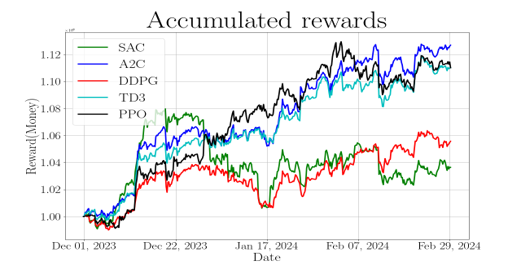
\includegraphics[width=.6\textwidth]{figures/Accumulated_Rewards_Reference.png}
        \caption{Performance of Reinforcement Learning Strategies on Financial Asset Trading \cite{RLinFinance}}
        \label{fig:Accumulated_Rewards_Reference}
\end{figure}

\subsection{Buy/Sell/Hold Agent}\label{sec:Model_Design:Buy_Sell_Hold_Agent}
The Buy/Sell/Hold (BSH) agent is designed to be the simplest trading agent possible.
The action space, described in Section \ref{sec:Model_Design:Buy_Sell_Hold_Agent:BSH_Action_Space}, is binary.
The reward function, described in Section \ref{sec:Model_Design:Buy_Sell_Hold_Agent:Position_Based_Reward_Function}, is based on the position of the agent at time $t$ and the change in closing price.

\subsubsection{BSH Action Space}\label{sec:Model_Design:Buy_Sell_Hold_Agent:BSH_Action_Space}
The BSH agent has a discrete action space as shown in table \ref{tab:Buy_Sell_Hold_Agent_Action_Space}.
The agent can choose to invest in cash or the asset at each time step.
Figure \ref{fig:Limit Order Action Plot Example} shows an example of the BSH action space.
Rising edges on the graph are buy signals and falling edges are sell signals.

\begin{table}[hbt!]
        \centering
        \begin{tabular}{||c|c||}
                \hline
                \textbf{Action} & \textbf{Description} \\
                \hline
                \hline
                0 & Invested in cash. \\
                \hline
                1 & Invested in asset. \\
                \hline
        \end{tabular}
        \caption{Buy/Sell/Hold Agent Action Space}
        \label{tab:Buy_Sell_Hold_Agent_Action_Space}
\end{table}

\begin{figure}[H]
        \centering
        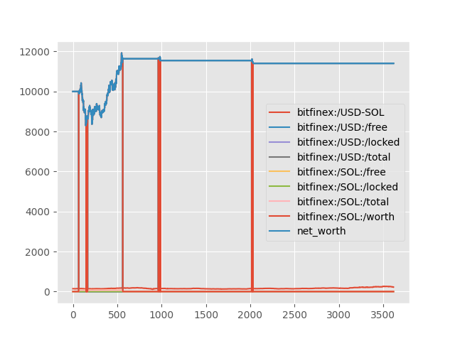
\includegraphics[width=.5\textwidth]{figures/BSH_Action_Example.png}
        \caption{BSH Action Plot Example}
        \label{fig:Limit Order Action Plot Example}
\end{figure}

\subsubsection{Position-Based Reward Function}\label{sec:Model_Design:Buy_Sell_Hold_Agent:Position_Based_Reward_Function}
The reward function for the BSH agent is based on the position of the agent ($x_t$) at time $t$ and the change in closing price ($Close_t$).
The reward function is shown in equation \ref{eq:Position_Based_Reward_Function} where $x_t$ is the position of the agent at time $t$.

\begin{equation}\label{eq:Position_Based_Reward_Function}
        R_t = \left(\text{Close}_{t} - \text{Close}_{t-1}\right) \cdot x_t
\end{equation}

\subsection{Managed Risk Agent}\label{sec:Model_Design:Managed_Risk_Agent}
The Managed Risk agent is designed to use limit orders to manage risk and maximize returns.
The action space, described in Section \ref{sec:Model_Design:Managed_Risk_Agent:Limit_Order_Action_Space}, is a combination of \textbf{stop loss}, \textbf{take profit}, and trade size values.
The reward function, described in Section \ref{sec:Model_Design:Managed_Risk_Agent:Sortino_Ratio_Reward_Function}, is based on the Sortino ratio which measures volatility as a function of downside risk.

\subsubsection{Limit Order Action Space}\label{sec:Model_Design:Managed_Risk_Agent:Limit_Order_Action_Space}
The Managed Risk agent has a discrete action space as shown in table \ref{tab:Limit_Order_Agent_Action_Space}.
Stop loss and take profit values are percentages at time $t$ relative to the change in closing price from the time a limit order was placed.
Stop loss values represent the maximum loss before selling and take profit values represent the maximum profit before selling.
Trade size values are fractions of the total account value.
Figure \ref{fig:Limit Order Action Plot Example} shows an example of the Managed Risk action space.

\begin{table}[hbt!]
        \centering
        \begin{tabular}{||c|c|c||}
                \hline
                \textbf{Action Parameter} & \textbf{Description} & \textbf{Values used} \\
                \hline
                \hline
                Stop Loss & Maximum loss before selling & [$2\%$, $5\%$, $10\%$] \\
                \hline
                Take Profit & Maximum profit before selling. & [$1\%$, $5\%$, $10\%$, $15\%$] \\
                \hline
                Trade Size & Size of next trade. & [$\frac{1}{16}$, $\frac{2}{16}$, \dots, $1$]\\
                \hline
        \end{tabular}
        \caption{Limit Order Agent Action Space}
        \label{tab:Limit_Order_Agent_Action_Space}
\end{table}

\begin{figure}[hbt!]
        \centering
        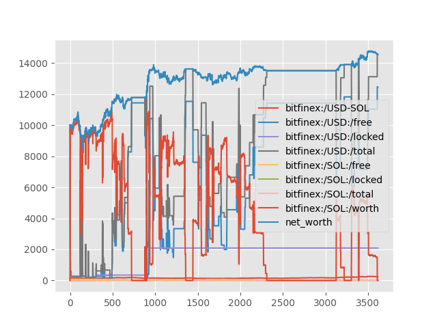
\includegraphics[width=.5\textwidth]{figures/Risk_action_example.png}
        \caption{Limit Order Action Plot Example}
        \label{fig:Limit Order Action Plot Example}
\end{figure}

\subsubsection{Sortino Ratio Reward Function}\label{sec:Model_Design:Managed_Risk_Agent:Sortino_Ratio_Reward_Function}
The reward function for the Managed Risk agent is based on the Sortino ratio which measures volatility as a function of downside risk \cite{sortino1994performance}.
The Sortino ratio is calculated using equation \ref{eq:Sortino_Ratio_Reward_Function} where $x_t$ is the position of the agent at time $t$, $r_f$ is the risk-free rate of return, and $\sigma_d$, shown in equation \ref{eq:Sortino_Ratio_Downside_Deviation}, is the standard deviation of all changes in price that are less than the risk free rate.

\begin{equation}\label{eq:Sortino_Ratio_Downside_Deviation}
        \sigma_d = \sqrt{\frac{1}{k} \sum_{i=0}^{k-1} \min\left(0, \text{Close}_{t-i} - \text{Close}_{t-i-1} - r_f\right)^2}
\end{equation}

\begin{equation}\label{eq:Sortino_Ratio_Reward_Function}
        R_t = \frac{\frac{x_{t} - x_{t-1}}{x_{t-1}} - r_f}{\sigma_d}
\end{equation}

\section{Implementation}\label{sec:Implementation}
The models described above were implemented in Python by leveraging third party libraries shown in table \ref{tab:3rd_Party_Libraries}.
NumPy and pandas were used for data manipulation.
pandas\_ta was leveraged for technical analysis calculations across pandas dataframes.
TensorTrade provides models for wallets, exchanges, assets, OpenAi Gym Environments, Reward Schemes, and Action Schemes as well as an API for accessing historical data from cryptocurrency exchanges.
Stable-Baseline3 provides a suite of reinforcement learning algorithms for training and testing agents.

\begin{table}[H]
        \centering
        \begin{tabular}{|c|c|}
                \hline
                \textbf{3rd Party Libraries} & \textbf{Usage} \\
                \hline
                \hline
                NumPy \cite{harris2020array} & Data manipulation and computations. \\
                \hline
                pandas \cite{reback2020pandas} & Data storage and manipulation. \\
                \hline
                pandas\_ta \cite{pandas-ta} & Technical Analysis computation. \\
                \hline
                TensorTrade \cite{Tensortrade} & Models for exchanges, assets, OpenAi Gym Environments. \\
                \hline
                stable\_baselines3 \cite{stable-baselines3} & Reinforcement Learning algorithm implementations. \\
                \hline
        \end{tabular}
        \caption{3rd Party Libraries}
        \label{tab:3rd_Party_Libraries}
\end{table}

\section{Analysis}\label{sec:Analysis}
To test the implementations, a python script was written following the implementation details above to train and test 100 BSH and Managed Risk models on 6 different cryptocurrencies and compare the results of the best models to baseline investment strategies.
The models were tested on Bitcoin (BTC) \cite{nakamoto2008bitcoin}, Ethereum (ETH) \cite{buterin2013ethereum}, 
Cardano (ADA) \cite{cardano2024}, Solana (SOL) \cite{yakovenko2017solana}, Litecoin (LTC) \cite{lee2011litecoin}, and Tron (TRX) \cite{sun2017tron} cryptocurrency markets with data from the Bitfinex exchange.

Some currencies had larger datasets than others due to the age of the cryptocurrency.
The models were split into train and test sets with the most recent $5$ months of data used for testing and the remainder of the data held for training.
Agents were given $\$10,000.00$ to start for training and testing.
Table \ref{tab:Train_and_Test_Sizes} shows the sizes of the train and test sets for each cryptocurrency.

\begin{table}[hbt!]
        \centering
        \begin{tabular}{||c|c|c||}
                \hline
                \textbf{Cryptocurrency} & \textbf{Training Set Size} & \textbf{Test Set Size} \\
                \hline
                \hline
                BTC & 53611 & 3673 \\
                \hline
                ETH & 53603 & 3673 \\
                \hline
                ADA & 18431 & 3673 \\
                \hline
                SOL & 18460 & 3673 \\
                \hline
                LTC & 52612 & 3673 \\
                \hline
                TRX & 52231 & 3618 \\
                \hline
        \end{tabular}
        \caption{Train and Test Sizes}
        \label{tab:Train_and_Test_Sizes}
\end{table}

The number of training steps was randomly selected from the list [$500$, $1000$, $5000$, $10000$, $15000$].
Each model's window size for PPO was randomly selected for the list [$96$, $72$, $48$, $24$, $12$].
Due to the lack of hard research providing standards for these values, random selection was used to allow for a variety of model results.
The best model performance on each cryptocurrency is shown in Figure \ref{fig:Results by Cryptocurrency}. 
Baseline investment strategies for investing in a savings account at $4\%$ interest or holding the asset for the entire period were plotted next to model results for comparison.
The number of training steps and window size for the best models are shown in Table \ref{tab:Best_Model_Hyperparameters}.

\begin{figure}[H]
        \centering
        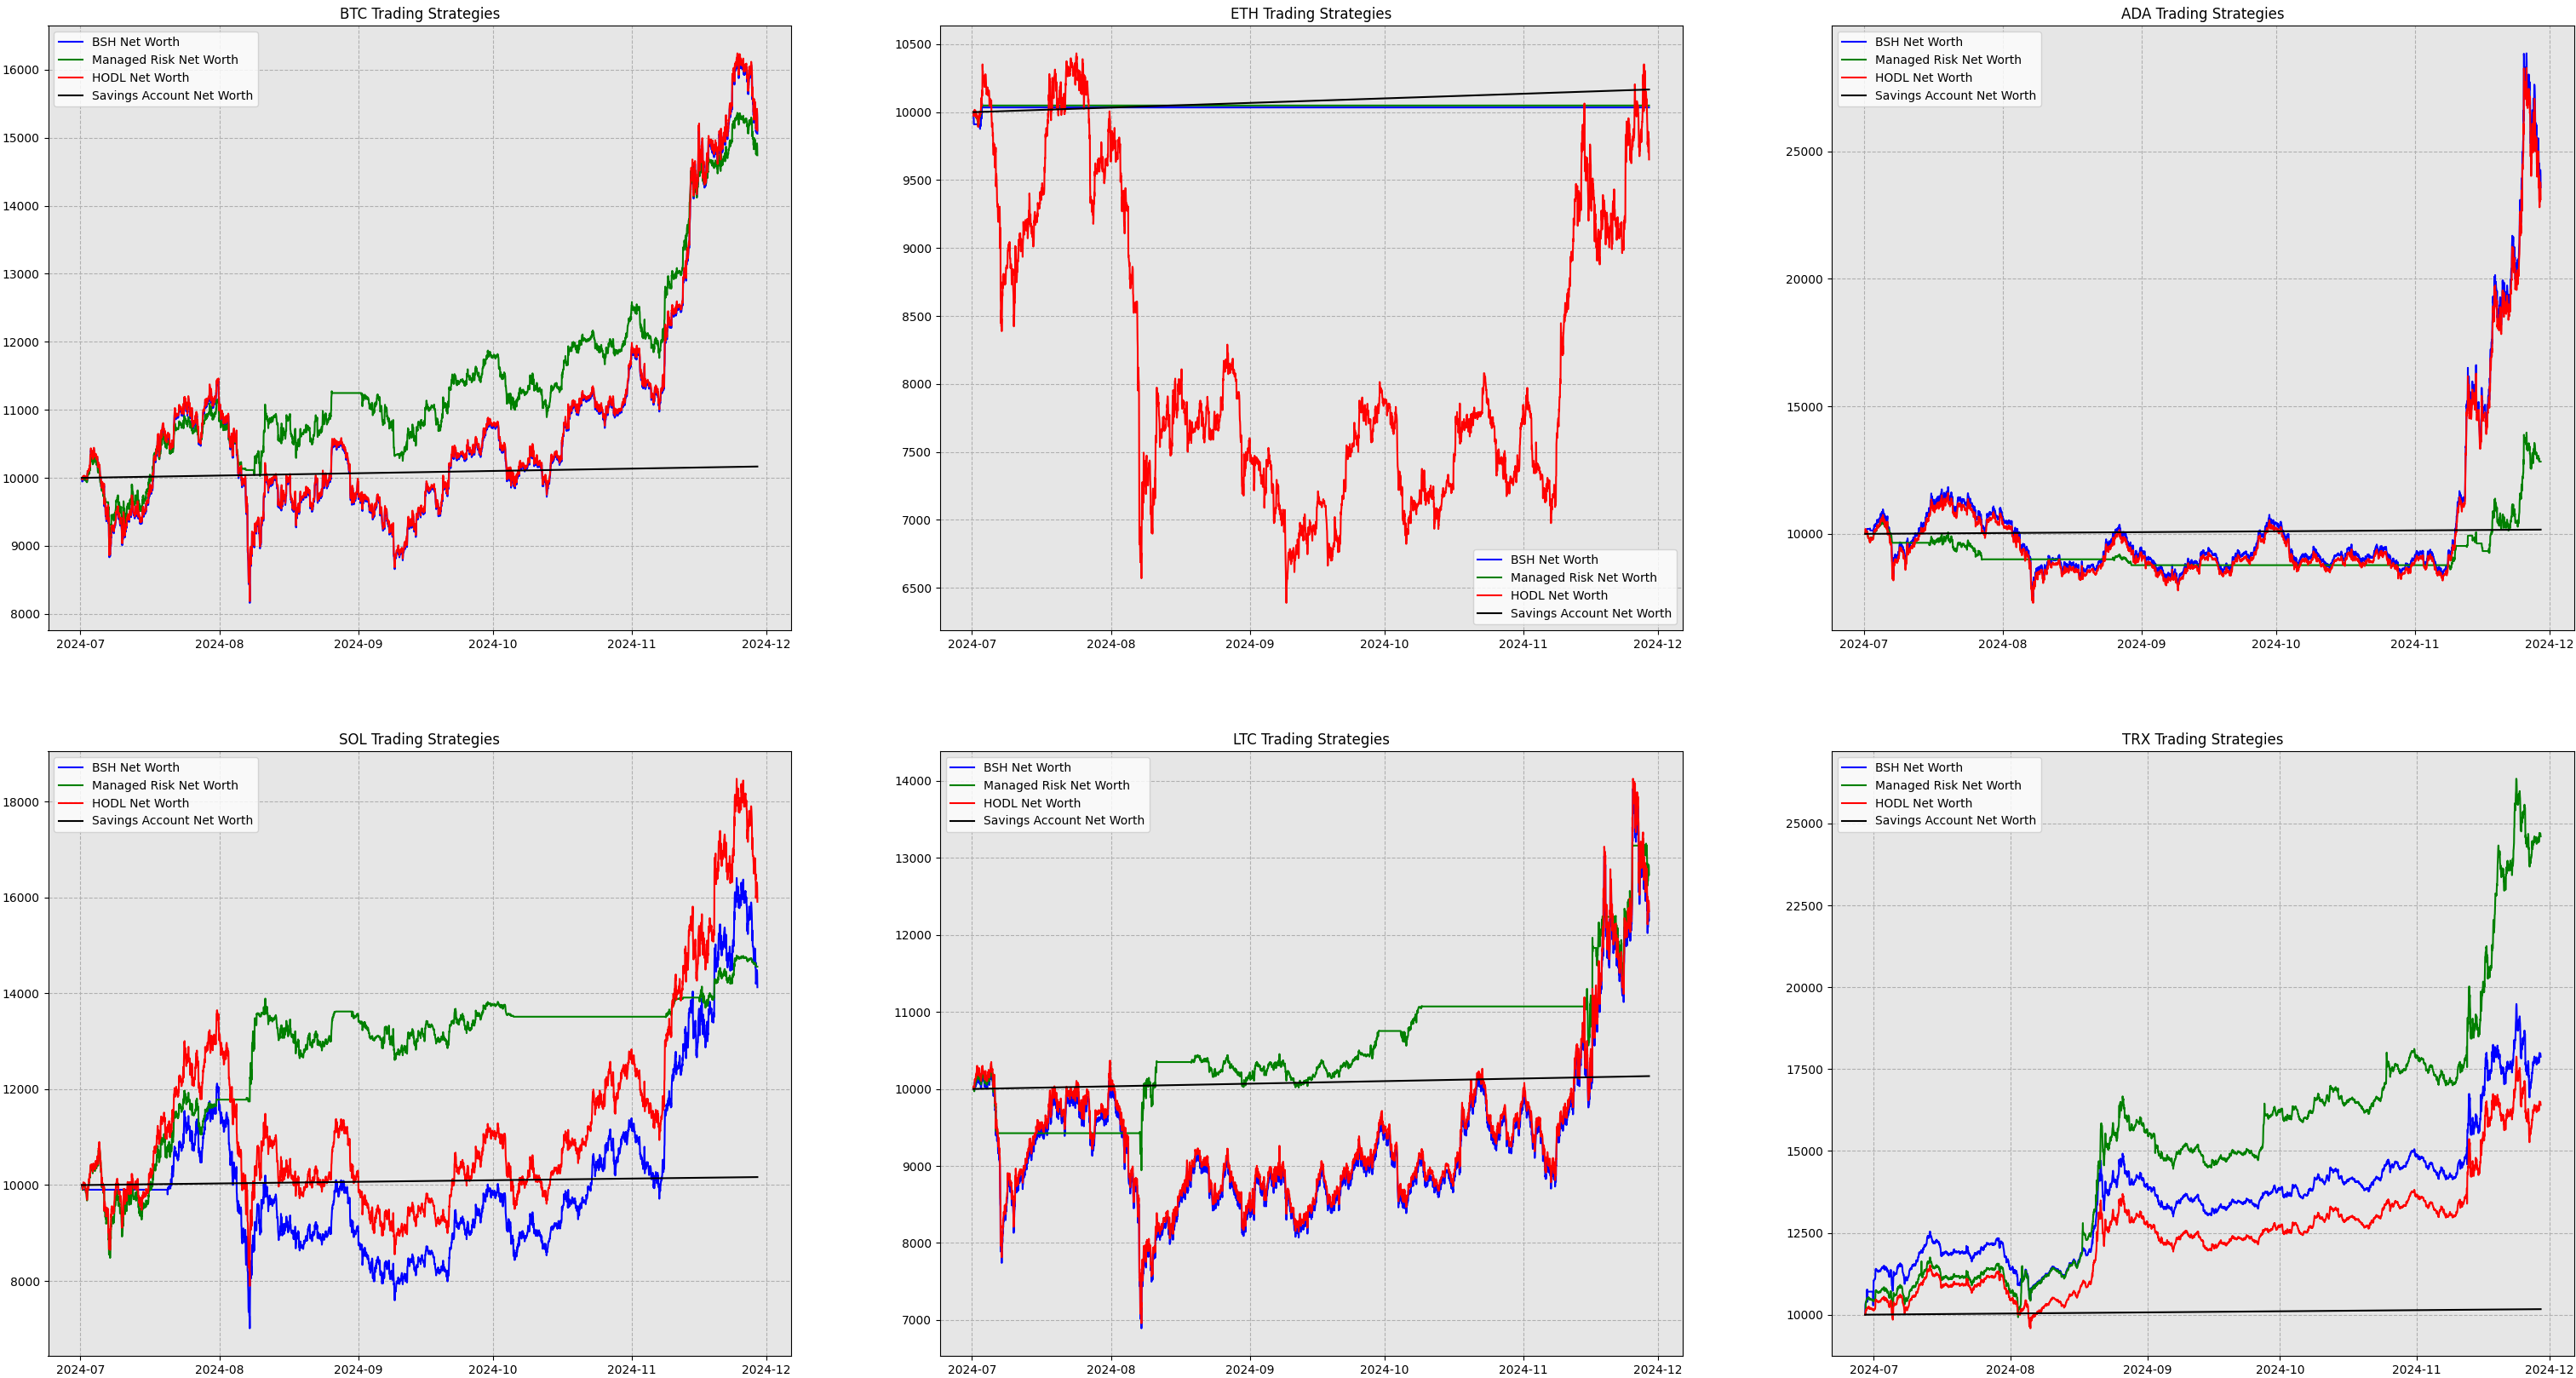
\includegraphics[width=\textwidth]{figures/model_results_per_asset.png}
        \caption{Results by Cryptocurrency. The green line is the Managed Risk model's performance. The blue line is the BSH model's performance. The red line is the net worth if the agent bought the asset and held the entire time. The black line is the performance of a savings account with $4\%$ interest.}
        \label{fig:Results by Cryptocurrency}
\end{figure}

\begin{table}[hbt!]
        \centering
        \begin{tabular}{||c|c|c|c|c||}
                \hline
                \textbf{Cryptocurrency} & $\text{BSH}_\text{training-steps}$ & $\text{BSH}_\text{window-size}$ & $\text{Managed Risk}_\text{training-steps}$ & $\text{Managed Risk}_\text{window-size}$ \\
                \hline
                \hline
                BTC & 500 & 96 & 15000 & 72 \\
                \hline
                ETH & 50000 & 48 & 500 & 12 \\
                \hline
                ADA & 1000 & 48 & 15000 & 12 \\
                \hline
                SOL & 500 & 96 & 15000 & 12 \\
                \hline
                LTC & 1000 & 72 & 500 & 72 \\
                \hline
                TRX & 5000 & 48 & 10000 & 24 \\
                \hline
        \end{tabular}
        \caption{Best Model Hyperparameters}
        \label{tab:Best_Model_Hyperparameters}
\end{table}

To compare the performance of the models across all cryptocurrencies, the results from Figure \ref{fig:Results by Cryptocurrency} were aggregated and plotted in Figure \ref{fig:Aggregate Results}.

\begin{figure}[H]
        \centering
        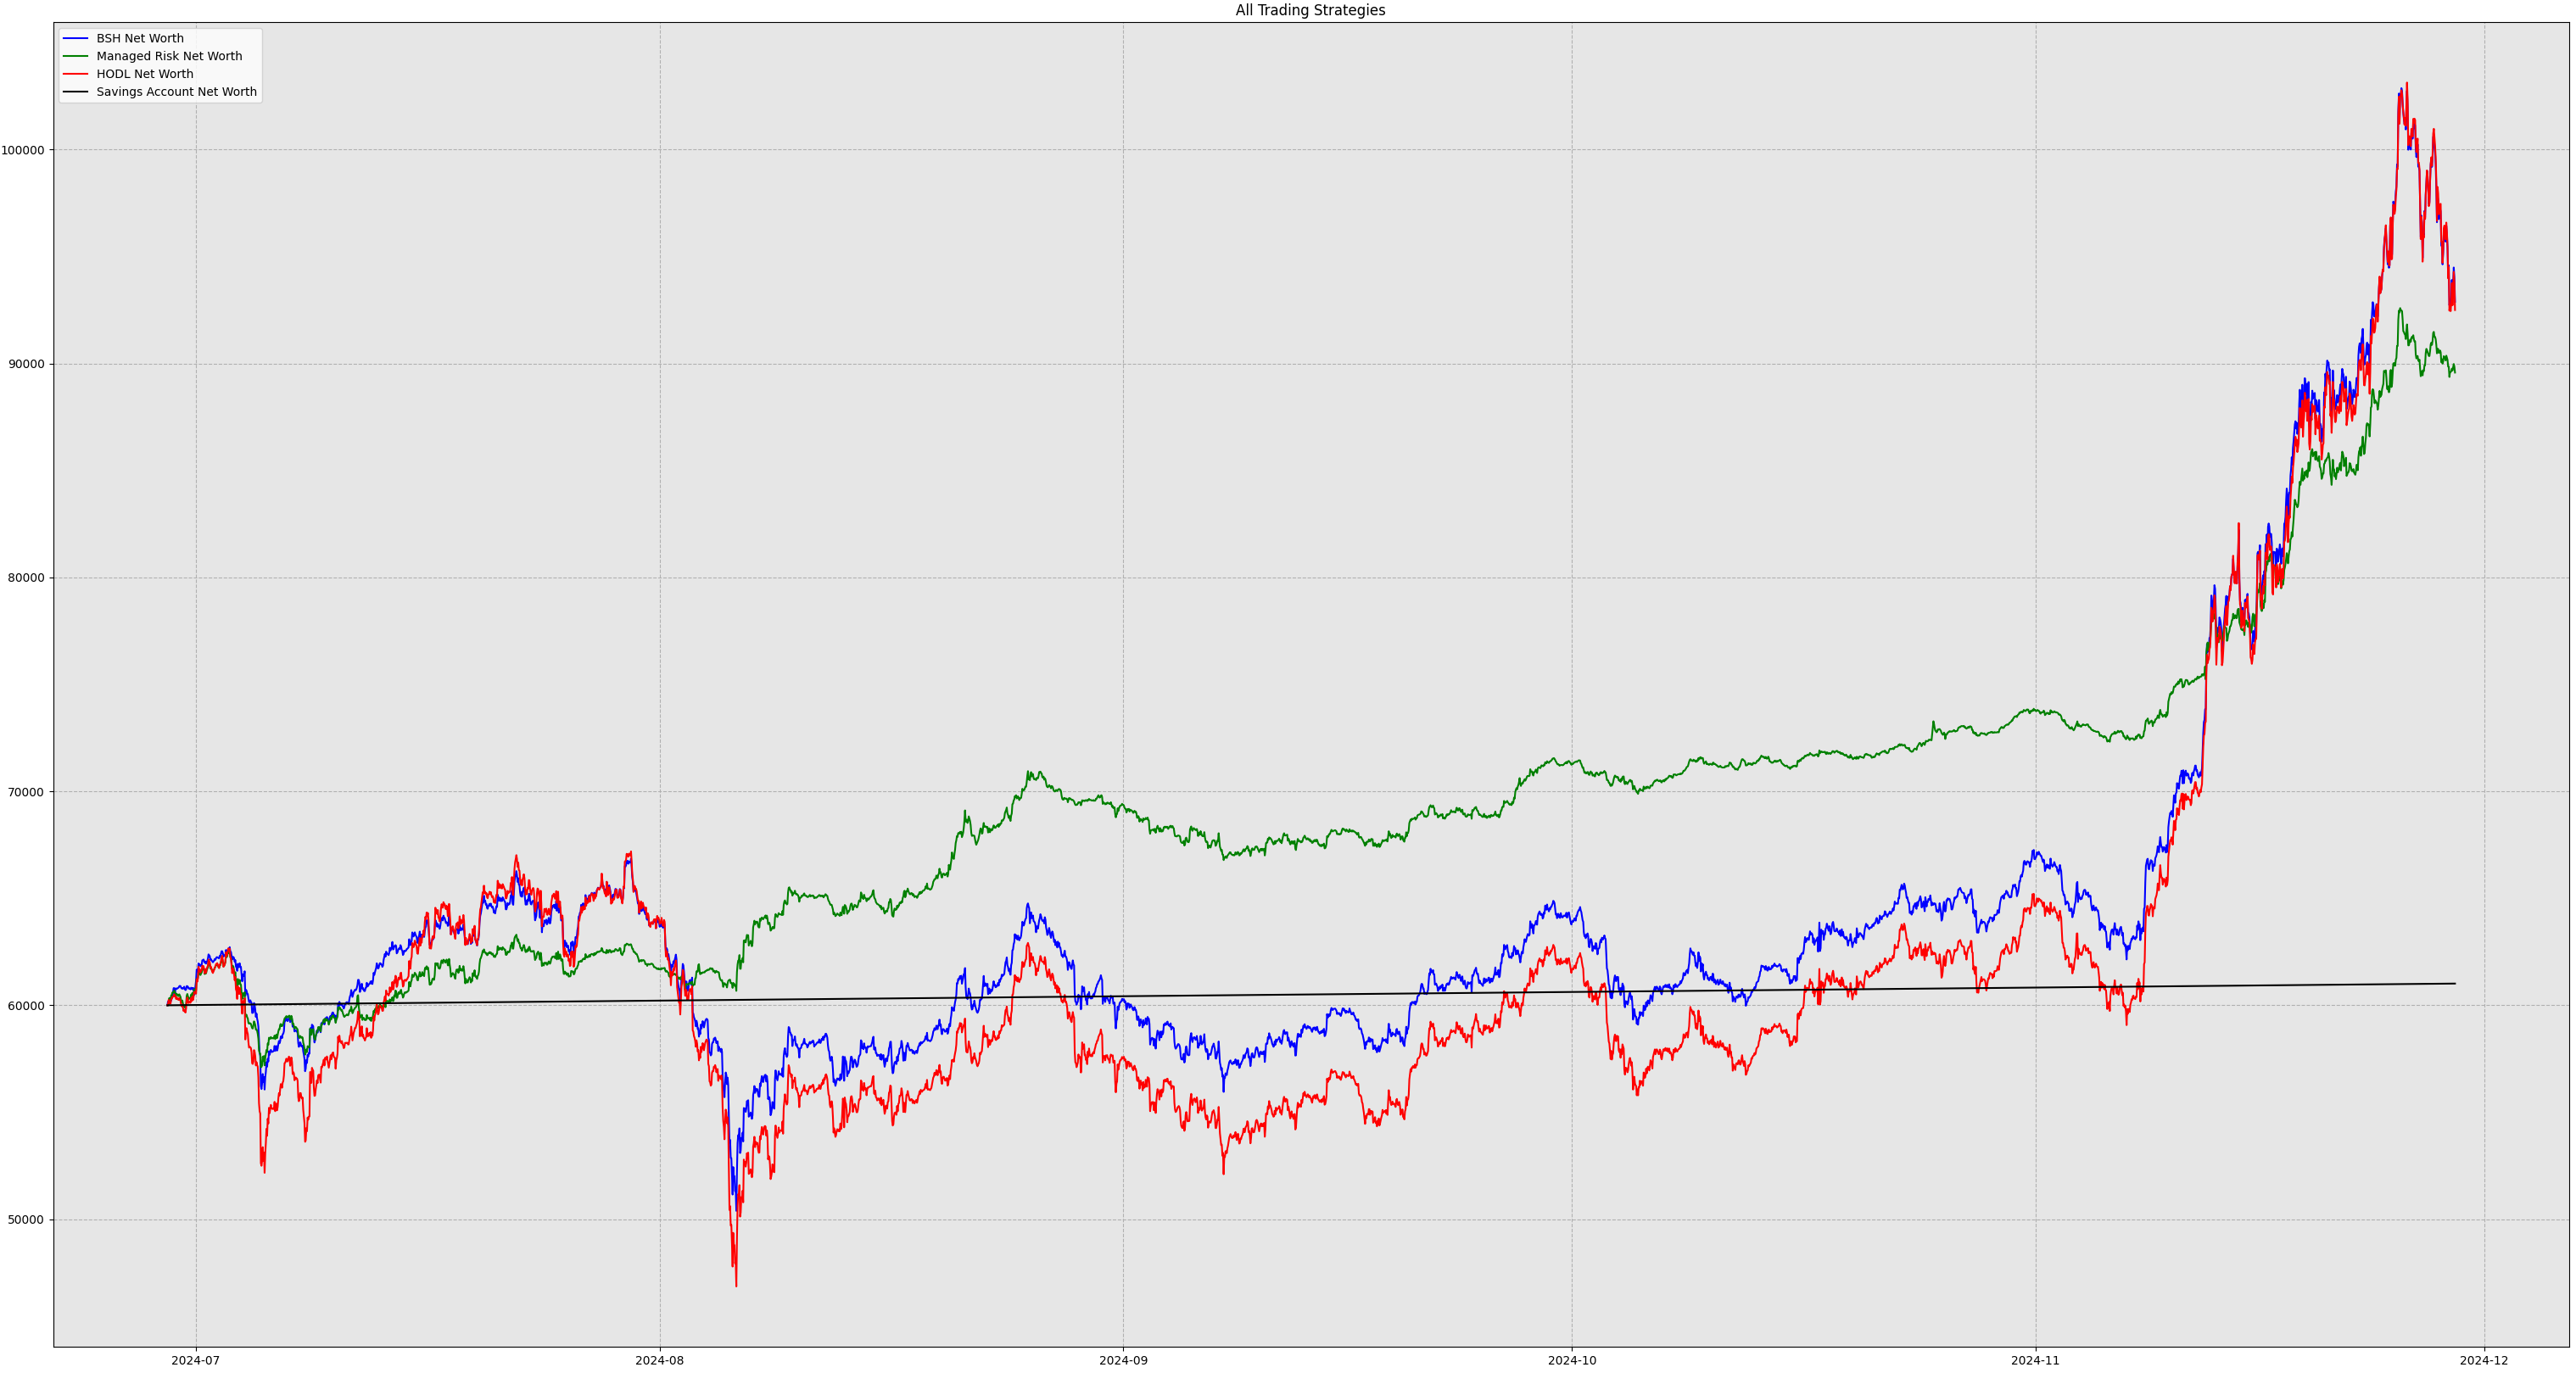
\includegraphics[width=.8\textwidth]{figures/aggregate_model_results.png}
        \caption{Aggregate Results. The green line is the Managed Risk model's performance. The blue like is the BSH model's performance. The red line is the net worth if the agent bought the asset and held the entire time. The black line is the performance of a savings account with $4\%$ interest.}
        \label{fig:Aggregate Results}
\end{figure}

\section{Discussion}\label{sec:Discussion}
The results show that, on average, the Managed Risk model performed better than the BSH model, holding the asset, or keeping the money in a high yield savings account.
The BSH model performed similarly, and slightly better, than holding the assets.
Since the BSH model followed the real price signal so closely, its success is likely secondary to the recent uptrend in price and not to the well placed market orders.
On the other hand, the Managed Risk model was able to protect the agent from large drops in price and take advantage of up trends in price.

\section{Future Work}\label{sec:Future_Work}
The models tested in this paper have room for improvement.
Currently, the feature space for the models is limited to a subset of technical analysis indicators.
Including fundamental analysis indicators and sentiment analysis could improve the performance.
Additionally, no feature ranking has been done to verify relevance of indicators.
Dimensionality reduction techniques like Principal Component Analysis (PCA) could help identify the most relevant features or be used as a transform to reduce feature space size and therefore reduce training time \cite{hotelling1933analysis}.

The models have been tested and deployed on a centralized exchange where the US Dollar (USD) is the base currency.
Another option would be to deploy on a decentralized token exchange where the base currency is a cryptocurrency such as Minswap \cite{nguyen2021mip}.
The fees on decentralized exchanges are typically lower and the prices are more volatile.
Since the Managed Risk models identify, and protecting from, large drops in price, it may perform well on one of these decentralized token exchanges.

\section*{Acknowledgements}\label{sec:Acknowledgements}
This work was performed as a final paper for the Foundations of Reinforcement Learning class at Johns Hopkins University taught by Professor Enrique Garcia Mallada.

\bibliography{pavlovBib}

\end{document}